\section{Resultados Energia}

\subsection{Ponte H}

A ponte H foi feita primeiramente em uma protoboard a fim de ser validada sua eficiência. Em seguida, o sistema foi transferido para a placa furada. O resistor utilizado apresentou mudança pois o item não estava disponível para a venda. Os resistores utilizados foram os 4 resistências de 560 $\Omega$. Dessa forma:  

\begin{center}
	$\frac{V_{cc} - V_{be}}{R}$ = $l_{b}$
	$\frac{3,3 - 0,7}{R}$ = 0,005\\
	R = 520$\Omega$\\
	$I_{ce}$ = 1000 $\Omega$ * 0,005 = 5 \textit{A}
\end{center}

\begin{itemize}
	\item Ib = corrente que aciona o transistor;
	\item $I_{ce}$ = corrente disponível à carga;
\end{itemize}

\begin{figure}[H]
	\centering
	\includegraphics[width=14cm]{figuras/ponteHpronta.png}
	\caption{Ponte H confeccionada. Fonte própria.}
	\label{ponteHpronta}
\end{figure}

Os integrantes que confeccionaram a placa tiveram dificuldades com a manipulação dos componentes, por não possuírem prática alguma com circuitos. Para posteriores trabalhos, é recomendado o uso de fios com bitolas maiores a fim de manter a segurança da ponte H.
Por fim, a ponte H foi integrada ao projeto da estufa com sucesso:

\begin{figure}[H]
	\centering
	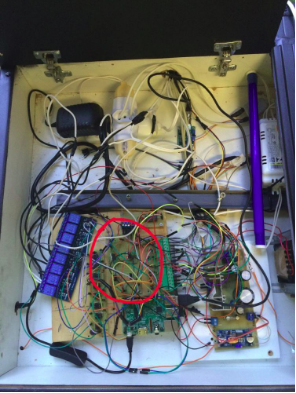
\includegraphics[width=14cm]{figuras/ponteHintegrada.png}
	\caption{Ponte H integrada ao projeto da estufa.}
	\label{ponteHintegrada}
\end{figure}


\subsection{Plantário}

No sistema que foi projetado para estufa, a área disponível para a locação da plantário foi restrita a 50cmx50cm. Visto que esse espaço ainda é compartilhado com os rolamentos da gaveta, a estrutura foi confeccionada em 3 tubos de PVC de 75mm de diâmetro e 40cm de comprimento. Além disso, foram feitos 2 furos em cada cano, com auxílio de serra-copo de 50mm de diâmetro, destinados a alojar as alfaces (as hortaliças do projeto). Os canos foram pintados de preto a fim de evitar o desenvolvimento de fungos e bactérias. O resultado é mostrado a seguir:

\begin{figure}[!htb]
	\centering
	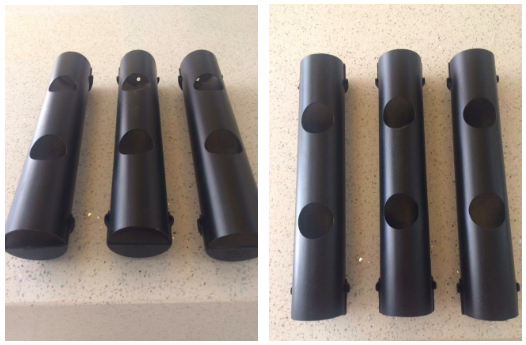
\includegraphics[width=14cm]{figuras/pvc.png}
	\caption{Plantário confeccionado com canos PVC. Fonte própria.}
	\label{pvc}
\end{figure}

Os coletores para alfaces foram feitos com acessórios de cabelo feminino. O resultado final integrado é mostrado a seguir:

\begin{figure}[!htb]
	\centering
	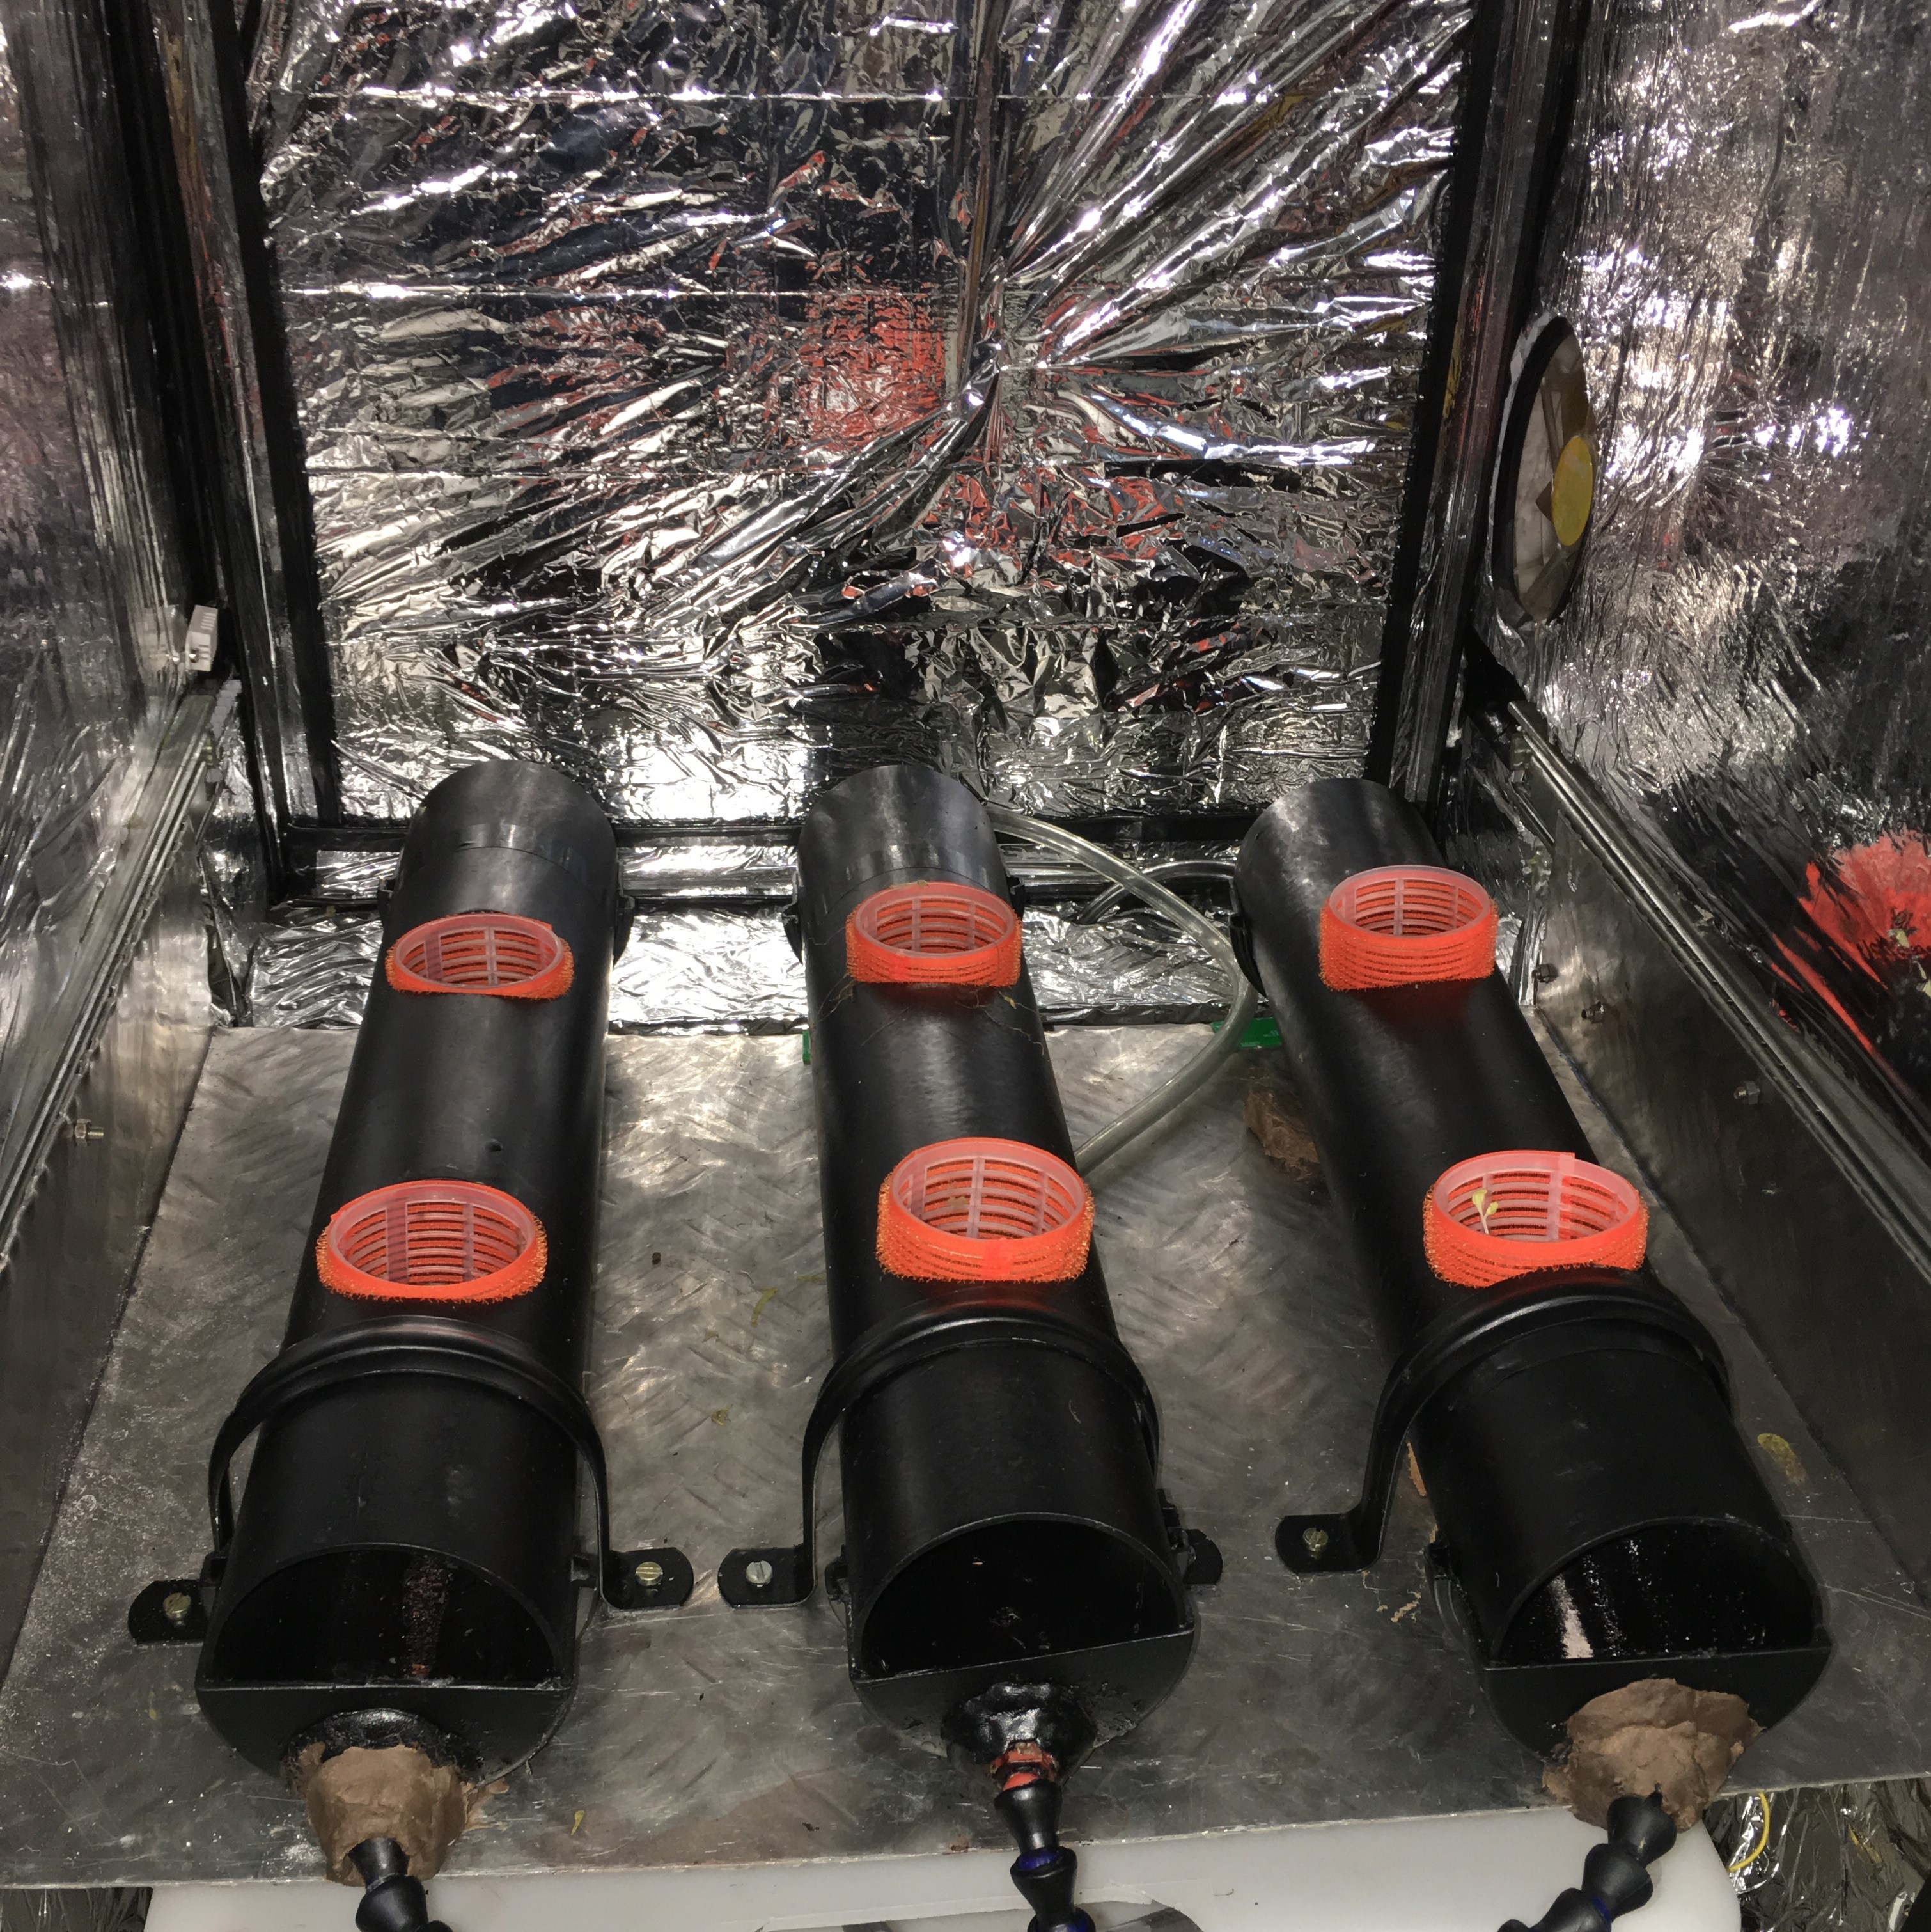
\includegraphics[width=14cm]{figuras/folha_aluminio.jpg}
	\caption{Plantário integrado.}
	\label{folha_aluminio}
\end{figure}


\subsection{Plantário}

Os coolers foram instaladas na estrutura, na parte superior e em sentidos opostos, a fim de garantir a circulação de fluído no interior e para fora.
O volume total do ambiente interno da estufa é dado por:

\begin{center}
	\large
	${\displaystyle V = b^2 * h = (0,5^2) * 0,7 = 0,175 m^3}$
\end{center}

Onde,

\begin{itemize}

	\item V= volume total ($m^{2}$);
	\item b= aresta da base quadrada (m);
	\item h= altura (m)
	
\end{itemize}

Dessa forma, o primeiro ventilador recicla esse mesmo volume em aproximadamente 16 segundos e o segundo o faz em aproximadamente 9 segundos.
A configuração final integrada é reportada a seguir:

\begin{figure}[!htb]
	\centering
	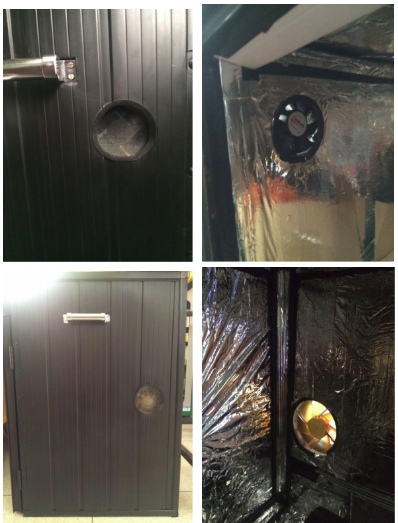
\includegraphics[width=14cm]{figuras/ventilacaoEstrutura.png}
	\caption{Ventilação pronta.}
	\label{ventilacaoEstrutura}
\end{figure}

\subsection{Fonte de alimentação}

O resultado obtido é reportado na imagem a seguir:

\begin{figure}[!htb]
	\centering
	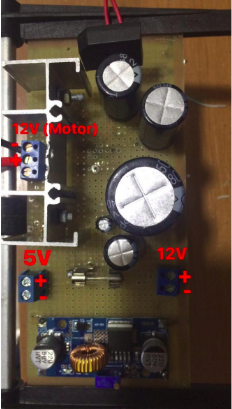
\includegraphics[width=7cm]{figuras/fonteDesen.png}
	\caption{Fonte desenvolvida.}
	\label{fonteDesen}
\end{figure}

As duas tensões de saída foram coletadas por meio de um osciloscópio:

\begin{figure}[!htb]
	\centering
	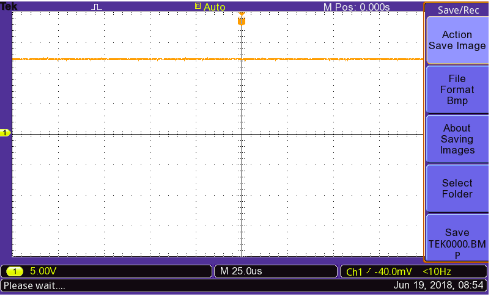
\includegraphics[width=14cm]{figuras/tensaoUm.png}
	\caption{Tensão de saída 1.}
	\label{tensaoUm}
\end{figure}

\begin{figure}[!htb]
	\centering
	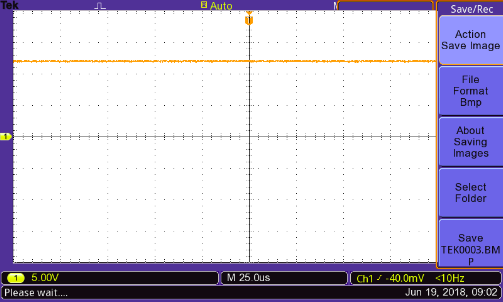
\includegraphics[width=14cm]{figuras/tensaoDois.png}
	\caption{Tensão de saída 2.}
	\label{tensaoDois}
\end{figure}

Os testes com carga foram feitos a partir de uma lâmpada incandescente 12V com pólos de 5W e 12W.

\begin{figure}[!htb]
	\centering
	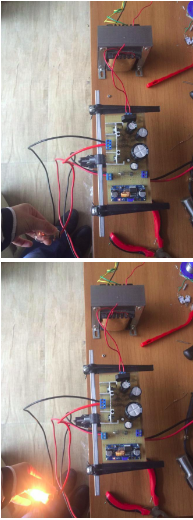
\includegraphics[width=7cm]{figuras/testeCarga.png}
	\caption{Teste de carga.}
	\label{testeCarga}
\end{figure}

Percebe-se nas imagens a seguir a variação do \textit{ripple} quando o circuito é fechado, sendo essa flutuação favorável.

\begin{figure}[!htb]
	\centering
	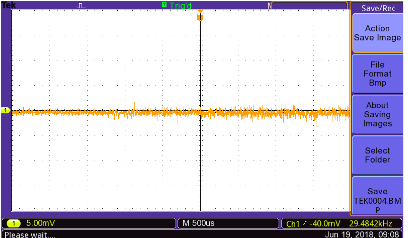
\includegraphics[width=14cm]{figuras/variacao1.png}
	\caption{Variação com carga na saída 1.}
	\label{variacao1}
\end{figure}

\begin{figure}[!htb]
	\centering
	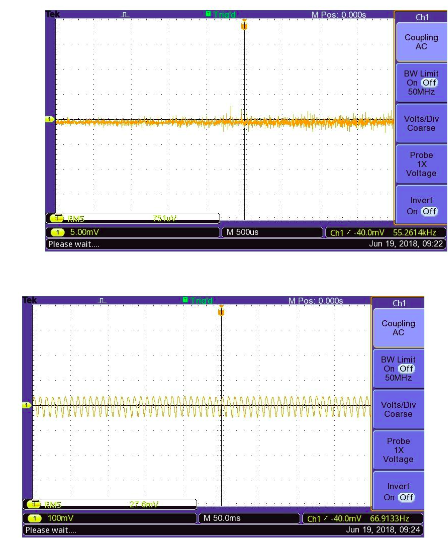
\includegraphics[width=14cm]{figuras/variacao2.png}
	\caption{Variação com carga na saída 2.}
	\label{variacao2}
\end{figure}

A diferença de comportamento entre as duas saídas pode ser justificada pela maior capacitância na primeira saída (capacitor na saída).
Por fim, a integração com a estufa foi realizada com sucesso como ilustrada na imagem a seguir:

\begin{figure}[!htb]
	\centering
	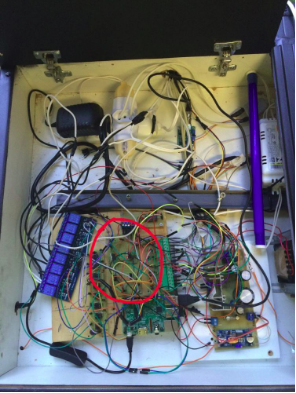
\includegraphics[width=14cm]{figuras/ponteHintegrada.png}
	\caption{ Fonte integrada ao projeto.}
	\label{ponteHintegrada}
\end{figure}

\subsection{Iluminação}

\begin{figure}[!htb]
	\centering
	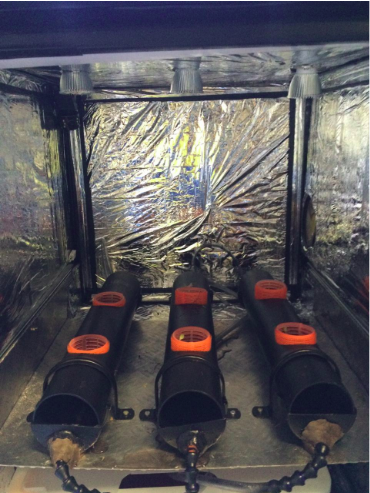
\includegraphics[width=14cm]{figuras/iluminaEstufa.png}
	\caption{Posição final.}
	\label{iluminaEstufa}
\end{figure}
